\documentclass{article}
\usepackage[utf8]{inputenc}
\usepackage[greek,english]{babel}
\usepackage{csquotes}
\usepackage{alphabeta}
\usepackage{amssymb}
\usepackage{tikz}
\usepackage[fleqn]{amsmath}
\usepackage{tabularx}
\usepackage{circledsteps}
\usepackage{extarrows}
\usepackage{mathtools}
\usepackage{lipsum}
\usepackage[linesnumbered, resetcount,algosection]{algorithm2e}
\usepackage{amsthm}
\newtheorem{theorem}{Theorem}[section]
\newtheorem{proposition}{Proposition}[theorem]
\newtheorem{corollary}{Corollary}[theorem]
\newtheorem{lemma}{Lemma}[theorem]
\newtheorem{properties}{Properties}[theorem]
\usepackage[sorting=none]{biblatex}
\definecolor{codegreen}{rgb}{0,0.6,0}
\definecolor{codegray}{rgb}{0.5,0.5,0.5}
\definecolor{codepurple}{rgb}{0.58,0,0.82}
\definecolor{backcolour}{rgb}{0.95,0.95,0.92}
\usepackage{listings}
\usepackage{chngcntr}
\usepackage{xcolor}
\usepackage{xspace}
\usepackage{float}
\usepackage{graphicx}
\usepackage{listingsutf8}
\usepackage{subfig}

\lstdefinestyle{mystyle}{
	inputencoding=utf8/latin1,
	backgroundcolor=\color{backcolour},   
	commentstyle=\color{codegreen},
	keywordstyle=\color{magenta},
	numberstyle=\tiny\color{codegray},
	stringstyle=\color{codepurple},
	basicstyle=\ttfamily\footnotesize,
	breakatwhitespace=false,         
	breaklines=true,                 
	captionpos=b,                    
	keepspaces=true,                 
	numbers=left,                    
	numbersep=5pt,                  
	showspaces=false,                
	showstringspaces=false,
	showtabs=false,                  
	tabsize=2
}

\lstset{style=mystyle}

\iffalse
\lstset{
	language=C,                % choose the language of the code
	numbers=left,                   % where to put the line-numbers
	stepnumber=1,                   % the step between two line-numbers.        
	numbersep=5pt,                  % how far the line-numbers are from the code
	backgroundcolor=\color{white},  % choose the background color. You must add \usepackage{color}
	showspaces=false,               % show spaces adding particular underscores
	showstringspaces=false,         % underline spaces within strings
	showtabs=false,                 % show tabs within strings adding particular underscores
	tabsize=2,                      % sets default tabsize to 2 spaces
	captionpos=b,                   % sets the caption-position to bottom
	breaklines=true,                % sets automatic line breaking
	breakatwhitespace=true,         % sets if automatic breaks should only happen at whitespace
	title=\lstname,                 % show the filename of files included with \lstinputlisting;
	style=mystyle
}
\fi

\lstset{inputpath={../Codes/}}

\graphicspath{ {../Images/} }

\title{OSLab 2023-24 | 1η Εργαστηριακή Άσκηση}
\author{Κόρδας Νικόλαος - Α.Μ.: 03121032 \\
	Κριθαρίδης Κωνσταντίνος - Α.Μ.: 03121045}
\date{29 Μαρτίου 2024}

\begin{document}
	\maketitle	
	
	\section{Ανάγνωση και εγγραφή αρχείων στη C και με τη βοήθεια κλήσεων συστήματος}
	Αρχικά, αντιγράψαμε τον φάκελο char-count στο home directory μας και στην συνέχεια τον μεταφέραμε με χρήση της scp στον προσωπικό μας υπολογιστή. Κατόπιν, ξεκινήσαμε να εξετάζουμε τον κώδικα που μας δόθηκε στο αρχείο a1.1-C.c. Διαπιστώνουμε πως το εκτελέσιμο που παράγεται από αυτό, ουσιαστικά, ανοίγει το αρχείο που του έχουμε περάσει ως πρώτο όρισμα προς ανάγνωση και το δεύτερο προς εγγραφή, με χρήση της fopen(). Το τρίτο όρισμα είναι ο χαρακτήρας που πρόκειται να αναζητήσει στο αρχείο. Στα παραπάνω ανοίγματα γίνονται και οι απαραίτητοι έλεγχοι αποτυχίας της εντολής. Κατόπιν, το πρόγραμμα διατρέχει ολόκληρο το πρώτο αρχείο, (μέχρι τον χαρακτήρα EOF) και με την χρήση της fgetc() διαβάζει έναν έναν τους χαρακτήρα τους ελέγχοντας αν είναι όμοιοι με τον χαρακτήρα που δόθηκε για ανάγνωση. Εάν είναι αυξάνει έναν μετρητή. Τέλος, εγγράφει το αποτέλεσμα στο δεύτερο αρχείο με την εντολή fprintf() και κλείνει τα δύο ανοιχτά αρχεία με την fclose(). \\
	
	\noindent Στόχος μας είναι να μιμηθούμε την παραπάνω λειτουργία αντικαθιστώντας την κλήση συναρτήσεων της βιβλιοθήκης της C με system calls. Με άλλα λόγια, να κάνουμε το πρόγραμμά μας linux specific. Ο κώδικάς μας γράφεται στο αρχείο a1.1-system\_calls.c ενώ το εκτελέσιμο που παράγεται είναι το a1.1-system\_calls. Κατά την κλήση του εκτελέσιμου παίρνουμε τα ίδια ορίσματα με παραπάνω. Έτσι, στον κώδικά μας, το πρώτο πράγμα που γίνεται είναι ο έλεγχος των ορισμάτων που δίνονται από τον χρήστη με την συνάρτηση argument\_handling(). Πιο συγκεκριμένα, αυτή η συνάρτηση ελέγχει εάν ο αριθμός των ορισμάτων είναι σωστός (ακριβώς 3 από τον χρήστη) και αν δόθηκε μόνο ένας χαρακτήρας προς αναζήτηση στο αρχείο. Στην συνέχεια, ορίζοντας τα κατάλληλα flags που απαιτούνται για την εγγραφή και την ανάγνωση των αρχείων, χρησιμοποιούμε την κλήση συστήματος open() η οποία επιστρέφει file descriptor (ακέραιο) για το κάθε αρχείο. Μετά, σύμφωνα και με τις διαφάνειες της εργασίας εκτελούμε την ανάγνωση του αρχείου που δόθηκε χαρακτήρα - χαρακτήρα και κάθε φορά που αυτός είναι όμοιος με αυτόν που δόθηκε προς εύρεση, αυξάνουμε έναν μετρητή κατά 1. Λεπτομερέστερα, η ανάγνωση πραγματοποιείται με τη βοήθεια ενός buffer (πίνακας χαρακτήρων 1024 byte) και της κλήσης συστήματος read(). Η read() σε κάθε επανάληψη του βρόχου διαβάζει μέχρι 1023 byte από το αρχείο, τα αποθηκεύει στον buffer, τον οποίο μετατρέπουμε σε συμβολοσειρά τοποθετώντας στο τέλος του τον χαρακτήρα '\textbackslash 0'. Διατρέχοντάς τον, μετράμε τις εμφανίσεις του c2c και ξανακάνουμε το ίδιο μέχρι να φτάσουμε στο τέλος του αρχείου (rcnt = 0, δηλαδή, η read() δε μπόρεσε να διαβάσει κανένα byte από το αρχείο). Μόλις λήξει η διαδικασία ανάγνωσης, κλείνουμε τον file descriptor του αρχείου αυτού με την κλήση συστήματος close(). Με την snprintf() τυπώνουμε το μήνυμα απόκρισής μας με τον αριθμό φορών που βρέθηκε ο c2c σε έναν buffer. Στην συνέχεια, αξιοποιούμε την κλήση συστήματος write() και τον κώδικα των διαφανειών για να γράψουμε το μήνυμα αυτό στο αρχείο που μας έδωσε ο χρήστης. Τέλος, κλείνουμε και αυτό το αρχείο και τερματίζουμε το προγραμμά μας. Αξίζει να σημειώσουμε πως κάθε κλήση συστήματος συνοδεύεται από τον κατάλληλο έλεγχο για την αποτυχία εκτέλεσής της. \\
	
	\noindent Ο κώδικας για το πρώτο μέρος της εργαστηριακής άσκησης φαίνεται παρακάτω: \\
	
	\lstinputlisting[language=C]{a1.1-system_calls.c}
	
	\section{Δημιουργία διεργασιών}
	Αυτή τη φορά παραθέτουμε πρώτα τον κώδικα της άσκησης διότι αυτός περιέχει απαντήσεις για όλα τα παρακάτω ερωτήματα. \\
	
	\lstinputlisting[language=C]{a1.2-fork.c}
	
	\subsection{Ερώτημα 1}
	Για να δημιουργήσουμε μία διεργασία παιδί καλούμε την συνάρτηση fork(). Συγκεκριμένα, η συνάρτηση αυτή επιστρέφει 0 στην διεργασία παιδί που δημιουργεί, το pid του παιδιού στον γονέα, ενώ την τιμή -1 σε περίπτωση αποτυχίας. Για αυτό μετά την κλήση της διακρίνουμε περιπτώσεις. \\
	
	\begin{itemize}
		\item Στην περίπτωση -1 εκτυπώνουμε μήνυμα λάθους.
		\item Στην περίπτωση 0 εκτελούμε τον κώδικα της διεργασίας παιδού που περιέχεται στην συνάρτηση child().
		\item Σε περίπτωση κάποιου αναγνωριστικού pid εκτελείται ο κώδικας της πατρικής διαδικασίας, parent().
	\end{itemize}
	
	\noindent Για το πρώτο ερώτημα, η child() απλά χαιρετάει τον κόσμο με ένα μήνυμα που αποθηκεύεται σε έναν buffer και τυπώνεται με την συνάρτηση print() την οποία έχουμε ορίσει εμείς και περιέχει τον κώδικα των διαφανειών για την κλήση συστήματος write(). Το μήνυμα που τυπώνει περιέχει το pid της και το pid της γονεϊκής διαδικασίας της. Προκειμένου να αποκτήσει το pid της χρησιμοποιεί την ρουτίνα getpid(), ενώ για του γονέα της την getppid(). Αντίστοιχα, ο γονέας περιμένει τον τερματισμό κάθε παιδιού του με την wait(), από την οποία λαμβάνει και το status του τερματισμού. Μόλις το παιδί τερματίσει εκτυπώνει ένα μήνυμα στην οθόνη που περιέχει το status αυτό αλλά και τον pid του παιδιού (Child process \%d exited with status \%d. \textbackslash n).
	
	\subsection{Ερώτημα 2}
	Στο ερώτημα αυτό ορίζουμε την μεταβλητή $x$ και της δίνουμε την τιμή 17 στον γονέα. Κατόπιν δημιουργούμε τα παιδιά. Κατά την δημιουργία τους, λόγω του copy on write, στιγμιαία έχουμε την ίδια τιμή και σε αυτά (17). Στην συνέχεια, όμως, εφόσον κάθε παιδί έχει το δικό του stack, ουσιαστικά, έχουμε αντιγραφή μόνο του ονόματος της μεταβλητής, αλλά όχι της πραγματικής υπόστασης της στη μνήμη. Για αυτό και όταν αλλάζει η τιμή της σε 42 από το παιδί, αυτό που βλέπουμε στην οθόνη δεν είναι πλέον η γονεϊκή τιμή 17, αλλά η νέα 42. Στην παρακάτω εικόνα φαίνεται το output αυτού του προγράμματος, για αυτό και το προηγούμενο ερώτημα.
	
	\begin{figure}[H]
		\centering
		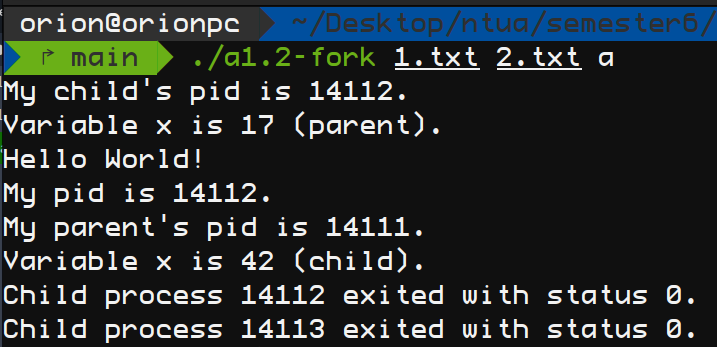
\includegraphics[scale = 0.45]{a1.2.png}
	\end{figure}
	
	\subsection{Ερώτημα 3}
	
	Η επέκταση που καλούμαστε να κάνουμε σε αυτό το ερώτημα αφορά την ανάθεση αναζήτησης του χαρακτήρα στην διεργασία παιδί. Ουσιαστικά, συμπληρώνουμε τον κώδικα της συνάρτησης child() με τον κώδικα a1.1-system\_calls.c. Το αρχείο ανοίγεται από την γονεϊκή διαδικασία και ο file descriptor περνιέται ως όρισμα στη συνάρτηση - παιδί. Η ανάγνωση γίνεται με τον ίδιο τρόπο, όπως και στην προηγούμενη άσκηση. Καθώς το παιδί και ο γονιός δεν επικοινωνούν (ακόμα) με κάποιο τρόπο μεταξύ τους, το παιδί αναλαμβάνει και το γράψιμο του αποτελέσματός του στο αρχείο που έχει επιλέξει ο χρήστης. Ο file descriptor του τελευταίου περνιέται και αυτός ως όρισμα στη συνάρτηση - παιδί. Ο κώδικας του parent() δεν αλλάζει και αυτό είναι λογικό, αφού η γονεϊκή διαδικασία δεν επωμίζεται επιπλέον αρμοδιότητες σε αυτό το ερώτημα και άρα συνεχίζει απλά να περιμένει το παιδί να ολοκληρώσει την ανάγνωση του αρχείου και να τερματίσει (wait()). 
	
	\subsection{Ερώτημα 4}
	
	Στο τελευταίο αυτό ερώτημα, αντί να συμπληρώνουμε τον κώδικα για την ανάγνωση του αρχείου (και την εγγραφή) στην συνάρτηση child(), επιλέγουμε να εκτελέσουμε απευθείας το εκτελέσιμο του κώδικα a1.1-system\_calls.c, του a1.1-system\_calls. Αυτό επιτυγχάνονται με την ρουτίνα execv(). Για να λειτουργήσει σωστά το εκτελέσιμο πρέπει να του περάσουμε τα ίδια ορίσματα με τα οποία κλήθηκε το a1.2-fork. Αυτό το επιτυγνάνουμε επίσης με την execv(). Η κλήση και η χρήση του προγράμματος πράγματι γίνεται με επιτυχία, όπως άλλωστε φαίνεται και στην εικόνα που παραθέσαμε παραπάνω.
	
	
	\section{Διαδιεργασική Επικοινωνία}
	
	Παραθέτουμε τον κώδικα και για αυτή την άσκηση πρώτα.
	
	\lstinputlisting[language=C]{a1.3-comm.c}
	
	\noindent Ο κώδικας αποτελεί επέκταση αυτού της 2ης άσκησης, όμως εδώ αντί ένα παιδί να διαβάζει το αρχείο, πολλά (P) παιδιά διαβάζουν το αρχείο παράλληλα. Τα παιδιά επικοινωνούν το πλήθος εμφανίσεων του χαρακτήρα που μέτρησαν στον γονέα τους, ο οποίος είναι υπεύθυνος να αθροίσει τις εμφανίσεις του χαρακτήρα στα τμήματα του αρχείου που διάβασε το κάθε παιδί και να εγγράψει στο αρχείο εξόδου το συνολικό πλήθος εμφανίσεων του χαρακτήρα αναζήτησης στο αρχείο εισόδου.\\
	\\
	Προσθέτουμε χειριστή του σήματος SIGINT που να τυπώνουν (όλες οι ενεργές διεργασίες) το πόσα παιδιά διαβάζουν το αρχείο. Βάζουμε sleep(1) μετά από κάθε εκτέλεση του χειριστή σήματος ώστε να μας δίνει το χρονικό περιθώριο να πατήσουμε το Ctrl+C πριν ολοκληρωθεί η εκτέλεση των διεργασιών. Εφόσον θέλουμε ο χειριστής να εκτελείται κάθε φορά που γίνεται Ctrl+C, πρέπει μέσα στη ρουτίνα εξυπηρέτησης της διακοπής να ξαναθέσουμε τον sigintHandler ως τον χειριστή του σήματος SIGINT.\\
	\\
	Ανοίγουμε το αρχείο εισόδου από τον γονέα πριν δημιουργήσει το παιδί, και άρα τα ανοιχτά αρχεία του παραμένουν ανοιχτά και για το παιδί. Μέσω του struct stat λαμβάνουμε το μέγεθος N του αρχείου σε bytes και χωρίζουμε βέλτιστα το αρχείο σε batches στα P παιδιά. Το P εδώ επιλέγεται να ισούται με τη σταθερά του προγράμματος CPUCORES = 8 για να διευκολύνεται η παραλληλη επεξεργασία. Το μέγεθος του batch είναι $\lfloor \frac{N}{P}\rfloor + 1$ για $0 \leq i < N - (P-1)\lfloor \frac{N}{P}\rfloor$ και $\lfloor \frac{N}{P}\rfloor$ για $N - (P-1)\lfloor \frac{N}{P}\rfloor \leq i < P$. Με αυτόν τον τρόπο, ελαχιστοποιούμε το μέγιστο μέγεθος batch για δεδομένο P, οπότε και τον μέγιστο χρόνο εκτέλεσης ενός παιδιού, με αποτέλεσμα να ελαχιστοποιείται και ο συνολικός χρόνος εκτέλεσης του αλγορίθμου.\\
	\\
	Για να γλιτώσουμε τον χρόνο ανοίγματος του αρχείου από το κάθε παιδί, ανοίγουμε το αρχείο μία φορά στον γονέα πριν δημιουργηθούν τα παιδιά, όπως εξηγήσαμε και πριν. Εκτός από τα ανοιχτά αρχεία, τα παιδιά μοιράζονται έτσι και τον δείκτη του πού βρίσκονται στο κάθε ανοιχτό αρχείο. Επιπλέον, παρότι τα παιδιά μπορούν να εκτελούνται παράλληλα, ο διάδρομος δεδομένων από και προς τον δίσκο είναι κοινός για όλες τις διεργασίες, δηλαδή τα read εκτελούνται στην πραγματικότητα σειριακά. Ακόμα, επειδή η κλήση συστήματος read είναι blocking, δεν υπάρχουν προβλήματα συγχρονισμού. Συμπερασματκά, μπορούμε να αναθέσουμε σε κάθε διεργασία να διαβάσει συγκεκριμένο πλήθος bytes ανάλογα με το batch size που της αναλογεί, χωρίς απαραίτητα αυτά να είναι ένα συνεχόμενο τμήμα του αρχείου που να έχουμε χωρίσει εξαρχής, καλώντας απλά τη read από το κάθε παιδί.\\
	\\
	Τέλος, η επικοινωνία από τα παιδιά προς τον γονέα για την μεταφορά της πληροφορίας του πλήθους εμφανίσεων του χαρακτήρα αναζήτησης στο αρχείο εισόδου γίνεται μέσω σωληνώσεων (pipes). Ο γονέας διατηρεί ένα πίνακα P θέσεων που στην κάθε θέση έχει έναν πίνακα 2 θέσεων που αντιστοιχεί στο pipe του με το αντίστοιχο παιδί. Αφού κάνουμε pipe τον κάθε πίνακα 2 θέσεων με την κλήση συστήματος pipe (και ελέγχοντας για σωστή εκτέλεση αφού δεν επιστρέφεται αρνητικός αριθμός), μετά το fork() κλείνουμε το άκρο του που δεν χρησιμοποιείται από την κάθε διεργασία. Για κάθε pipe, στη θέση 1 (άκρο εγγραφής) γράφει το παιδί και από τη θέση 0 (άκρο ανάγνωσης) διαβάζει ο γονέας. Αφού ολοκληρωθεί η επικοινωνία του γονέα με ένα παιδί, και οι 2 διεργασίες κλείνουν τα εναπομείναντα ανοιχτά άκρα του pipe τους. Το τελικό αποτέλεσμα το συγκεντρώνει ο γονέας και το γράφει στο αρχείο εξόδου.
	
	\section{Εφαρμογή παράλληλης καταμέτρησης χαρακτήρων}
	
	Ξεκινάμε πάλι παρουσίαζοντας τον κώδικα της άσκησης. Παρόλα αυτά, επειδή χωρίζεται σε πολλά αρχεία και έχει μεγάλο μέγεθος, παραθέτουμε αρχικά μόνο τις main και τις δηλώσεις συναρτήσεων κάθε αρχείου. Ο πλήρης κώδικας μπορεί να βρεθεί στο παράρτημα στο τέλος της αναφοράς.
	
	\lstinputlisting[language=C]{config.h}
	
	\lstinputlisting[language=C, firstline=1, lastline=68, caption={Main body of frontend}]{a1.4-frontend.c}
	
	\lstinputlisting[language=C, firstline=1, lastline=143, caption={Main body of dispatcher}]{a1.4-dispatcher.c}
	
	\lstinputlisting[language=C, firstline=1, lastline=58, caption={Main body of worker}]{a1.4-worker.c}
	
	\begin{figure}[H]
		\centering
		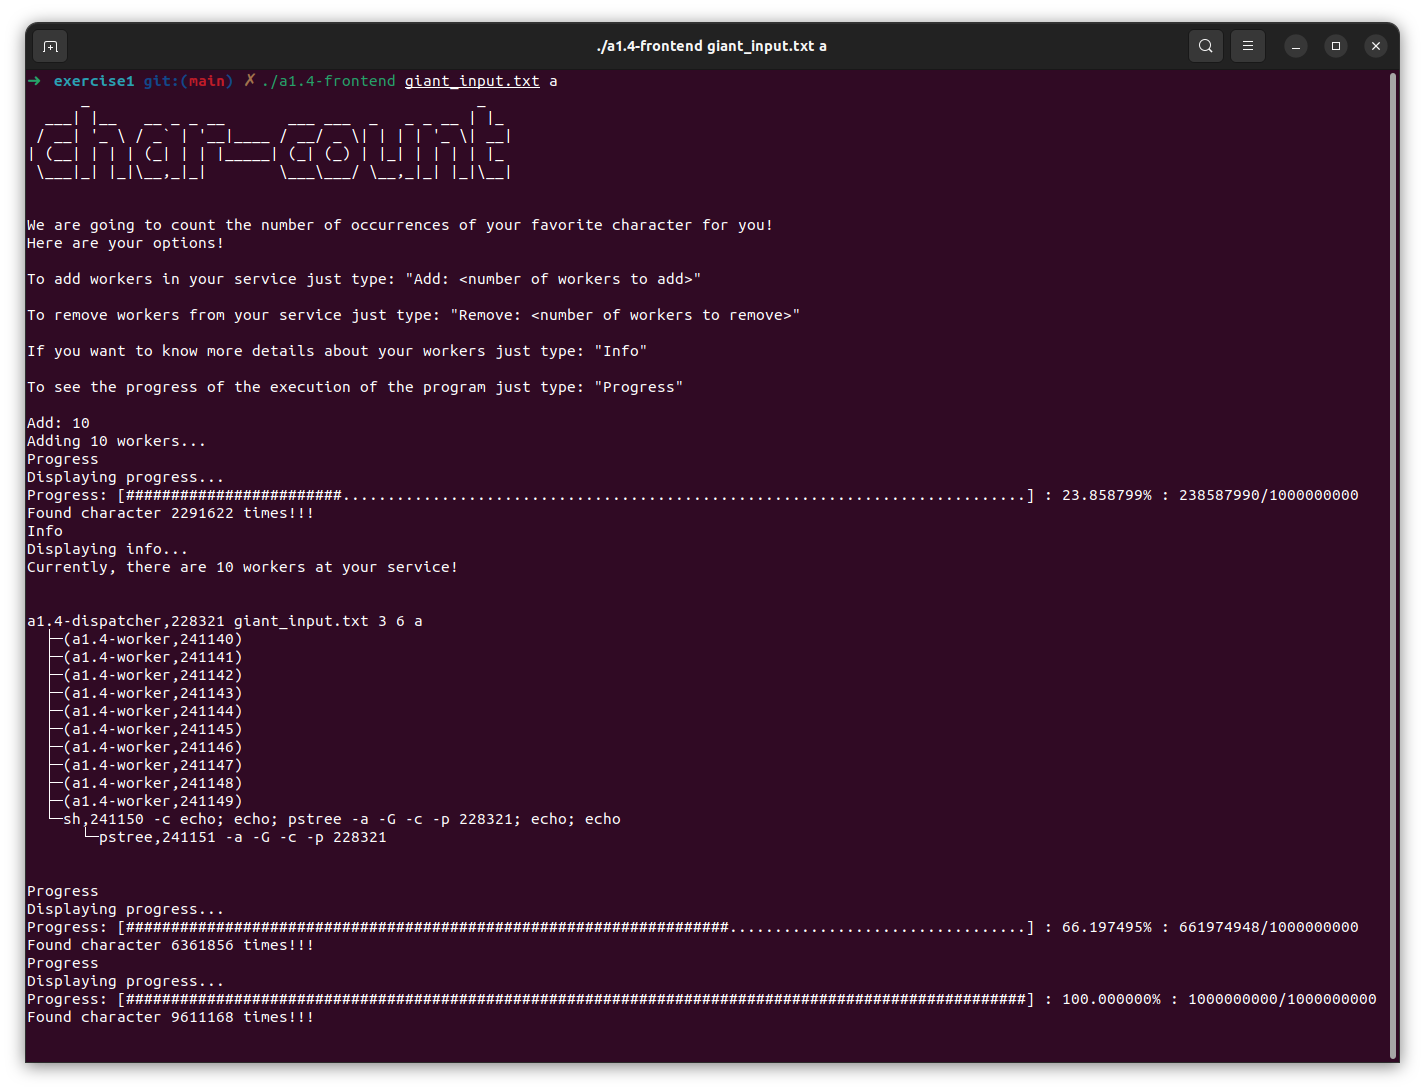
\includegraphics[width=\textwidth]{a1.4_Execution.png}
		\caption{Παράδειγμα εκτέλεσης της εφαρμογής με πολύ μεγάλο αρχείο εισόδου}
	\end{figure}
	
	Η εφαρμογή χωρίζεται σε 3 δομικά στοιχεία: το frontend, τον dispatcher και τους workers.\\
	\\
	Το frontend λειτουργεί ως διεπαφή του χρήστη με την εφαρμογή. Αρχικά τυπώνει το welcome message με οδηγίες χρήσης της εφαρμογής. Δέχεται 4 εντολές:
	\begin{itemize}
		\item Add: $<$number of workers to add$>$
		\item Remove: $<$number of workers to remove$>$
		\item Info
		\item Progress
	\end{itemize}
	
\end{document}
